\documentclass[border=4pt]{standalone}
\usepackage{tikz}
\usetikzlibrary{positioning, arrows.meta, calc, fit, backgrounds}
\begin{document}
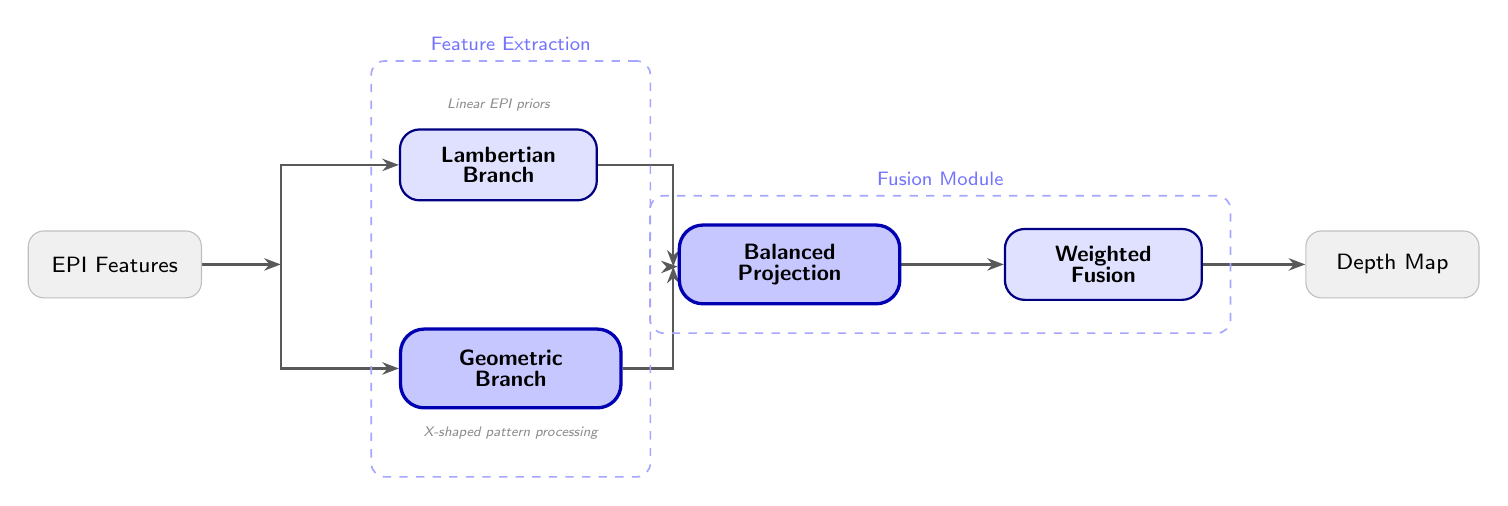
\begin{tikzpicture}[
  input/.style={draw, rounded corners=2mm, minimum width=2.2cm, minimum height=0.85cm,
                fill=gray!12, draw=gray!50, align=center, font=\sffamily\footnotesize},
  module/.style={draw, rounded corners=2.5mm, minimum width=2.5cm, minimum height=0.9cm,
                 fill=blue!12, draw=blue!50!black, line width=0.8pt, align=center,
                 font=\sffamily\footnotesize\bfseries},
  innov/.style={draw, rounded corners=3mm, minimum width=2.8cm, minimum height=1.0cm,
                fill=blue!22, draw=blue!70!black, line width=1.2pt, align=center,
                font=\sffamily\footnotesize\bfseries},
  output/.style={draw, rounded corners=2mm, minimum width=2.2cm, minimum height=0.85cm,
                 fill=gray!12, draw=gray!50, align=center, font=\sffamily\footnotesize},
  arr/.style={-{Stealth[length=6pt]}, thick, color=black!65},
  gbox/.style={draw=blue!35, dashed, rounded corners=5pt, inner sep=10pt,
               line width=0.6pt},
  ann/.style={font=\sffamily\tiny\itshape, text=black!45},
]

% Input
\node[input] (input) {EPI Features};

% Split point
\coordinate[right=1.0cm of input] (split);

% Lambertian Branch (top)
\node[module, above right=0.8cm and 1.5cm of split] (lambert)
  {Lambertian\\[-2pt]Branch};

% Geometric Branch (bottom, innovation)
\node[innov, below right=0.8cm and 1.5cm of split] (geometric)
  {Geometric\\[-2pt]Branch};

% Annotations near branches
\node[ann, above=0.1cm of lambert] (lann) {Linear EPI priors};
\node[ann, below=0.1cm of geometric] (gann) {X-shaped pattern processing};

% Midpoint between branches
\path (lambert) -- (geometric) coordinate[midway] (midbranch);

% Balanced Projection (innovation)
\node[innov, right=2.2cm of midbranch] (bproj)
  {Balanced\\[-2pt]Projection};

% Merge coordinate
\coordinate (merge) at ($(lambert.east)!0.5!(geometric.east) + (0.8,0)$);

% Weighted Fusion
\node[module, right=1.3cm of bproj] (fusion)
  {Weighted\\[-2pt]Fusion};

% Output
\node[output, right=1.3cm of fusion] (output) {Depth Map};

% Arrows
\begin{scope}[on background layer]
  \draw[arr] (input) -- (split);
  \draw[arr] (split) |- (lambert);
  \draw[arr] (split) |- (geometric);
  \draw[arr] (lambert.east) -| (merge);
  \draw[arr] (geometric.east) -| (merge);
  \draw[arr] (merge) -- (bproj);
  \draw[arr] (bproj) -- (fusion);
  \draw[arr] (fusion) -- (output);
\end{scope}

% Group Boxes
\begin{scope}[on background layer]
  \node[gbox, fit=(lambert)(geometric)(lann)(gann),
        label={[font=\sffamily\scriptsize, text=blue!55]above:Feature Extraction}] {};
  \node[gbox, fit=(bproj)(fusion),
        label={[font=\sffamily\scriptsize, text=blue!55]above:Fusion Module}] {};
\end{scope}

\end{tikzpicture}
\end{document}